%%%%%%%%%%%%%%%%%%%%%%%%%%%%%%%%%%%%%%%%%%%%%%%%%%%%%%%%%%%%%%%%%%%%%%%%%%%%%%%%%%%%%%
% author                : louis tomczyk
% date of production    : 2024-12-05
% licence               : cc-by-nc-sa
%                         Attribution - Non-Commercial - Share Alike 4.0 International
%%%%%%%%%%%%%%%%%%%%%%%%%%%%%%%%%%%%%%%%%%%%%%%%%%%%%%%%%%%%%%%%%%%%%%%%%%%%%%%%%%%%%%

\documentclass[tikz,border=5mm]{standalone}
\usepackage{pgfmath}

\begin{document}

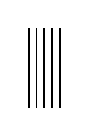
\begin{tikzpicture}[scale=1]
    \pgfmathsetmacro{\spacing}{0.1}     % Pas du réseau
    \pgfmathsetmacro{\rectWidth}{0.01}  % Largeur des fentes
    \pgfmathsetmacro{\angleRot}{0}   % angle de rotation
    \pgfmathsetmacro{\nSlits}{5}       % nombre de fentes
    \pgfmathsetmacro{\ymax}{1}          % Hauteur des fentes

    % Calcul du centre pour la rotation
    \pgfmathsetmacro{\xmin}{\spacing}   % Coordonnée minimale en x
    \pgfmathsetmacro{\xmax}{1}          % Coordonnée maximale en x
    \pgfmathsetmacro{\xcenter}{(\xmin+\xmax)/2}
    \pgfmathsetmacro{\ycenter}{\ymax/2}

    % Appliquer la rotation
    \begin{scope}[rotate=\angleRot,shift={(\xcenter,\ycenter)}]
        \foreach \i in {1,...,\nSlits}{
            \pgfmathsetmacro{\x}{\xmin + \i * \spacing}
            \draw[fill=black] (\x-\xcenter-\rectWidth/2, 0-\ycenter) rectangle ++(\rectWidth, \ymax);
        }
    \end{scope}
\end{tikzpicture}

\end{document}
